
  A partir da análise conceitual dos métodos e metodologias para construção de ontologias presentes na sessão anterior, 
  o método escolhido para a realização deste projeto, levando em conta as etapas/fases propostas por cada uma dessas 
  metodologias ou métodos no que tange ao processo de construção de ontologias, foi o método \textit{\textbf{Ontology 101}}.
  
  Os aspectos observados na escolha do método foram: \textbf{a)} suporte literário bem consolidado e disponível 
  (livros, artigos, guias e etc); \textbf{b)} o método é baseado na literatura do paradigma orientado a objetos;
  \textbf{c)} familiarização por parte dos integrantes do grupo com os conceitos e processos propostos pelo método.

\vspace{0.5cm}
  
{\raggedright
  \textit{\textbf{Ontology 101}}.
}
  
  De acordo com Breitman (\citeyear{breitman05}), o processo de construção de uma ontologia a partir do método 101,
  resumidamente, envolve as seguintes etapas:
  \begin{itemize}
   \item Definição das classes dessa ontologia;
   \item Disposição das classes em uma hierarquia taxonômica;
   \item Definição de propriedades e valores para os mesmos;
   \item Preenchimento dos valores das propriedades para cada instância.
  \end{itemize}
  
  \begin{figure}[!htb]
    \centering
    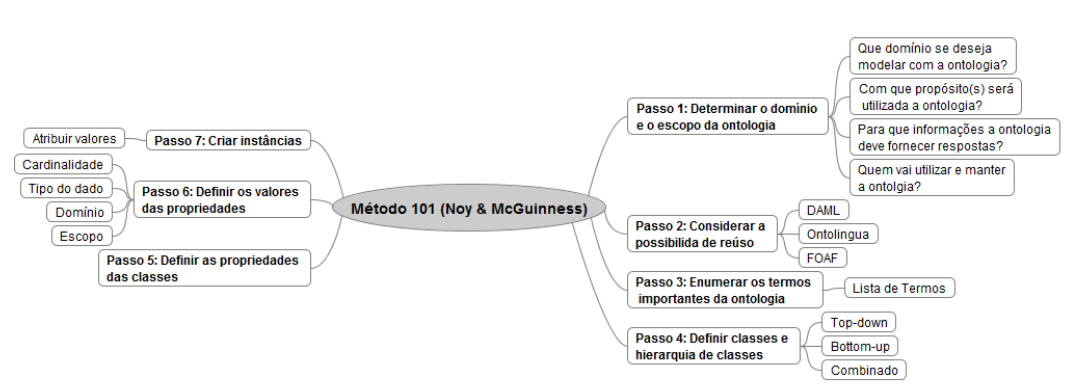
\includegraphics[scale = 0.4]{101-Web}
    \caption[Método 101 para construção de ontologia]{Método 101 para construção de ontologias. Fonte: \cite{bortolato14}}
    \label{fig:101-Web}
  \end{figure}
  
  A Figura \ref{fig:101-Web} ilustra um esquemático do método 101 no qual é detalhado cada um dos seus sete passos.
  
\vspace{0.5cm}  
  
{\raggedright  
  \textbf{1º Passo: Determinar o domínio e o escopo da ontologia}
}
  
  Para se determinar o domínio e o escopo da ontologia, Natalya F. Noy e Deborah McGuinness sugerem os seguintes questionamentos
  \cite{breitman05}:
  
  \begin{itemize}
   \item Que domínio se deseja cobrir com a ontologia?
   \item Com que protótipo(s) será utilizada a ontologia?
   \item Para que informações a ontologia deve fornecer respostas?
   \item Quem vai utilizar e manter a ontologia?
  \end{itemize}
  
  Segundo Breitman (\citeyear{breitman05}), estas perguntas servirão para avaliar a ontologia após sua conclusão.
  
\vspace{0.5cm}  
  
{\raggedright  
  \textbf{2º Passo: Considerar o reúso de outras ontologias}
}
  
  É importante considerar os termos que alguém já codificou em uma ontologia e se é possível refinar ou reutilizar
  modelos existentes para o domínio de nossa própria aplicação. Várias ontologias estão disponíveis eletronicamente,
  podendo ser facilmente importadas para editores e ambientes de desenvolvimento. \cite{breitman05}
  
  Atualmente existem várias bibliotecas de ontologias que disponibilizam modelos para reúso. As bibliotecas do projeto
  Ontolingua, DAML e KACTUS, por exemplo, disponibilizam um grande número de ontologias que podem ser reutilizadas, refinadas
  ou adaptadas. \cite{breitman05}
  
\vspace{0.5cm}  
  
{\raggedright  
  \textbf{3º Passo: Enumerar os termos importantes da ontologia}
}
  
  É útil fazer uma lista de todos os termos que deseja-se definir ou explicar aos usuários. Quais termos gostaríamos de abordar? 
  Quais propriedades terão esses termos? O que gostaríamos de dizer sobre esses termos? É importante obter uma lista compreensiva 
  de termos sem se preocupar com a redundância entre os conceitos que eles representam, relacionamentos entre termos ou qualquer 
  propriedade que eles venham a ter. \cite{noy15}
  
\vspace{0.5cm}  
  
{\raggedright  
  \textbf{4º Passo: Definir classes e a hierarquia de classes}
}
  
  Segundo Noy e McGuinness (\citeyear{noy15}), definir as classes e a hierarquia entre elas e definir  suas propriedades (5º Passo)
  são feitos de forma paralela,  pois seria difícil fazer um após o outro. O curso natural, na prática, é definir uma classe e 
  descrever suas propriedades logo após.
  
  Existem muitas abordagens possíveis para se fazer uma hierarquia de classes: \cite{breitman05}
  
  \begin{itemize}
   \item A abordagem \textbf{topo-para-baixo} (\textit{top-down}) inicia-se com a definição dos conceitos mais gerais do domínio (pai ou superclasse) 
   e, posteriormente, esses conceitos são especializados em conceitos mais específicos (filhos ou subclasses). Essa abordagem é 
   conhecida, também, como decomposição funcional. 
   \item A abordagem \textbf{baixo-para-cima} (\textit{bottom-up}), pelo contrário, inicia-se com a definição dos conceitos mais específicos 
   (filhos ou subclasses) com o subsequente agrupamento dessas classes em conceitos mais gerais (pai ou superclasse). Esses
   agrupamentos são organizados de acordo com uma estratégia de generalização. \cite{noy15}
   \item A \textbf{Combinação} (\textit{middle-out}) é a conjunção das abordagens descritas anteriormente. Primeiramente, são definidos
   os conceitos mais notórios e então esses são especializados e generalizados adequadamente. \cite{noy15}
  \end{itemize}
  
  De acordo com Noy e McGuinness (\citeyear{noy15}), nenhuma das três abordagens é a melhor a ser utilizada, isso vai depender da visão
  pessoal do modelador do domínio. Geralmente, a \textbf{combinação} tende a ser a mais utilizada pelos desenvolvedores de ontologia,
  uma vez que os conceitos mais centrais são mais descritivos no domínio da ontologia. \cite{noy15}
  
\vspace{0.5cm}  
  
{\raggedright  
  \textbf{5º Passo: Definir as propriedades das classes}
}
  
  Segundo Noy e McGuinness (\citeyear{noy15}), as classes sozinhas não proveem subsídios suficientes para responder as questões de competência
  do 1º Passo (Determinar o domínio e o escopo da ontologia). Para isso é necessário criar uma estrutura interna de seus conceitos.
  
  No passo anterior (Definir classes e a hierarquia das classes) já fora selecionadas as classes obtidas dos termos que foram listados
  no 3º Passo (Enumerar os termos importantes da ontologia).  Muito dos termos remanescentes, provavelmente, representaram as
  propriedades das classes. Para cada propriedade deve-se determinar qual(ais) classe(s) este(s) descreve(m). \cite{noy15}
  
  De acordo com Noy e McGuinness (\citeyear{noy15}), existem vários tipos de propriedades relativas a classes: intrínsecas, 
  extrínsecas, partes, relacionamentos com classes e objetos, entre outras. Todas as subclasses ou filhos de uma classe 
  (pai ou superclasse) herdam suas propriedades.
  
\vspace{0.5cm}  
\pagebreak
  
{\raggedright
  \textbf{6º Passo: Definir os valores das propriedades}
}
  
  “Propriedades podem assumir diferentes valores, dependendo da expressividade da linguagem de ontologia que está sendo utilizada”
  \cite{breitman05}. Um exemplo é a cardinalidade.
  
  Alguns sistemas permitem cardinalidade única (um único valor) entre as propriedades e ostros permitem cardinalidade múltipla 
  (propriedades multivaloradas). \cite{noy15}
  
  Na liguagem OWL, por exemplo, é permitido utilizar tipos de dados no preenchimento dos valores das propriedades. \cite{breitman05}
  
{\raggedright  
  Aqui está uma lista dos tipos de dados mais comuns:
}
  
  \begin{itemize}
   \item Cadeia de caracteres (\textit{String});
   \item Números ( Às vezes valores mais específicos de ponto flutuante (\textit{Float}) e inteiros são usados);
   \item Booleanos;
   \item Listas enumeradas de elementos.
  \end{itemize}
  
\vspace{0.5cm}  

{\raggedright  
\textbf{7º Passo: Criar instâncias}
}

  O último passo é criar instâncias individuais das classes na hierarquia. Definir uma instância de uma classe consistem em:
  (1) Escolher a classe; 
  (2) Criar uma instância individual dessa classe; 
  (3) Preencher os valores de suas propriedades. \cite{noy15}
  